
\documentclass[12pt]{book}

\usepackage[utf8]{inputenc}
\usepackage[T1]{fontenc}
\usepackage{geometry}
\usepackage{graphicx}
\usepackage[spanish, es-tabla]{babel}
\usepackage{amsthm}
\usepackage{amsmath}
\usepackage{trfsigns}
\usepackage{amssymb}
\usepackage{caption}

\DeclareCaptionType{equ}[][]
%\captionsetup[equ]{labelformat=empty}

%Para listado de programas
\usepackage{listings}
\usepackage{color}

\definecolor{mygreen}{rgb}{0,0.5,0}
\definecolor{mygray}{rgb}{0.7,0.7,0.7}
\definecolor{mymauve}{rgb}{0.58,0,0.82}

\lstset{ %
	 backgroundcolor=\color{mygray},   % choose the background color; you must add \usepackage{color} or \usepackage{xcolor}
	 basicstyle=\footnotesize\ttfamily,        % the size of the fonts that are used for the code
	 breaklines=true,            % Zeilen werden Umgebrochen
	 keywordstyle=\color{red},
	 commentstyle=\itshape\color{mygreen},    % comment style
	 numbers=left,                    % where to put the line-numbers; possible values are (none, left, right)
	 numbersep=5pt                   % how far the line-numbers are from the code
}



\newtheorem{thm}{Teorema}[section]
\theoremstyle{definition}
\newtheorem{dfn}{Definición}[section]
\theoremstyle{remark}
\newtheorem{note}{Nota}[section]
\theoremstyle{plain}
\newtheorem{lem}[thm]{Lema}

\geometry{letterpaper}



%un estilo propio
\usepackage{fancyhdr}
\setlength{\headheight}{15pt}

\pagestyle{fancy}
\renewcommand{\chaptermark}[1]{ \markboth{\chaptername\ \thechapter: #1}{} }
\renewcommand{\sectionmark}[1]{ \markright{ Sección \thesection. #1}{} }

\fancyhf{}
\fancyhead[LE,RO]{\thepage}
\fancyhead[RE]{\textit{ \nouppercase{\leftmark}} }
\fancyhead[LO]{\textit{ \nouppercase{\rightmark}} }
\fancyfoot[CE]{\textit{\textcopyright 2021 Departamento de I+D\\
		SMARTEST} }
\fancyfoot[CO]{\textit{Departamento de I+D, SMARTEST \\
		Elaboró: Dr. Casimiro Gómez González} }	            
\fancypagestyle{plain}{ %
	\fancyhf{} % remove everything
	\renewcommand{\headrulewidth}{0pt} % remove lines as well
	\renewcommand{\footrulewidth}{0pt}
}



\title{Percepción Remota}
\author{Dr. Casimiro Gómez González\\
	Departamento de I+D, SMARTEST\\
               correo: casimiro.gomez@smartest.mx\\
               Tel: 222 707 4118}
\date{Otoño 2021}

\begin{document}
\frontmatter
\maketitle


\chapter{Prólogo}

La Percepción Remota es una disciplina basada en ciencia y  tecnología que permite  desarrollar, capturar, procesar y analizar imágenes, junto con otros datos físicos de la Tierra, obtenidos  desde sensores en el espacio, sensores aerotransportados y con sensores que capturan datos de mediciones in situ.


La información adquirida con detectores a bordo de
satélites o aviones ha resultado de gran utilidad para
muchas y diferentes aplicaciones: agricultura,
minería, fenómenos naturales, detección de aguas
contaminadas; asimismo para el monitoreo de
bosques y de glaciares, entre otras.
A la técnica que nos permite adquirir información de
un objeto o fenómeno sin estar en contacto con él se
le conoce como percepción remota. Este término se
utiliza comúnmente para referirse a la observación de
nuestro planeta a través de cámaras y otros tipos de
sensores, como los radares y las cámaras térmicas,
montados, como ya mencionamos, en aviones o
satélites.
Las imágenes satelitales tienen diferentes
características. Estas dependen de los sensores o
detectores con las que son obtenidas. No es lo
mismo una cámara en el visible que en el infrarrojo,
por ejemplo. Esto es importante ya que la aplicación
específica, el uso que se les dará, depende de estas
peculiaridades.
Las principales características de las imágenes
satelitales se describen a continuación:
Resolución espacial. Ésta corresponde al área sobre
la Tierra que cubre cada pixel de la imagen. Por
ejemplo, las imágenes obtenidas con los satélites
GOES de la Administración Nacional Oceánica y
Atmosférica (NOAA, por sus siglas en inglés) de los
Estados Unidos tienen una resolución espacial de un
kilómetro cuadrado. Con imágenes de esta resolución
espacial es posible analizar el clima a nivel regional,
por ejemplo, en todo México.
Existen, desde luego, imágenes de mayor resolución,
como las tomadas con el satélite comercial
RapidEye, en las que un pixel cubre cinco metros
cuadrados de área de la Tierra, Se utilizan para
estudios de cobertura de suelo, monitoreo de
inundaciones o para determinar el daño a cultivos
provocado por inundaciones o granizo. Existen
imágenes aún con mayor resolución, algunos
satélites las obtienen con una resolución espacial de
61 centímetros cuadrados, con la cual es posible
trabajar en aplicaciones de catastro o aquellas que
involucran la identificación de estructuras.
Resolución espectral. Es importante conocer otras
características de los sensores utilizados en los
satélites, como son la región y ancho de banda del
espectro electromagnético que pueden registrar, ya que ellas determinan la resolución espectral de la
imagen. El espectro electromagnético va desde los
rayos gamma (longitudes de onda cortas, frecuencias
altas), los rayos X, la luz ultravioleta, luz visible (a la
que el ojo humano es sensible y se compone de las
bandas rojo, verde y azul), los rayos infrarrojos, las
microondas y radiofrecuencia (longitudes de onda
largas, frecuencias cortas). Algunos de los sensores
registran radiación electromagnética en el intervalo
del visible (como las cámaras digitales), el infrarrojo
(cercano infrarrojo y térmico), mientras que otros
registran microondas, como los radares.
Las imágenes multi-espectrales están compuestas
por varias bandas en el espectro electromagnético.
Existen satélites que tienen una combinación de
bandas del visible e infrarrojo. La combinación de
bandas es determinante en el tipo de aplicaciones
que se les da a las mismas. Por ejemplo, podemos
utilizar las imágenes en el visible para identificar
estructuras, y una combinación de bandas del visible
y el cercano infrarrojo son ideales para identificar
vegetación. Con las imágenes de radar es posible
identificar estructuras aún de noche o cuando existe
nubosidad y lluvia.
Resolución temporal. Cada determinado tiempo
podemos obtener una imagen del mismo lugar con el
mismo satélite, esto nos define la resolución temporal
de la imagen satelital. La periodicidad con la que se
pueden obtener las imágenes es una característica
relevante, ya que de este periodo de tiempo depende
la capacidad que tendremos para detectar cambios
en esa región. Estos cambios sirven para identificar
zonas deforestadas, la evolución de una inundación y
el progreso de un cultivo, entre otras.
Resolución radiométrica. En una imagen satelital, la
señal registrada por cada pixel de cada banda
representa un valor de la luz reflejada por el área del
objeto que cubre. La cantidad de valores diferentes
para representar un pixel de la imagen nos define la
resolución radiométrica de la imagen.

Con los valores de estas características podemos
darnos una idea de las aplicaciones de percepción
remota en las que las podemos utilizar. Una de las
problemáticas más importantes en las que
históricamente se ha aplicado la percepción remota,
son los fenómenos naturales. Existen mecanismos
internacionales para facilitar ayuda a una nación
cuando le ocurre un desastre. Al país afectado se le
proporcionan imágenes satelitales de manera gratuita
y si éste, por alguna razón, no tiene la capacidad de
procesarla, también se presta ayuda para dicho
procesamiento y se les entregan los productos
derivados: mapas temáticos, que se utilizan para
tomar decisiones en casos de inundaciones,
terremotos, maremotos, huracanes, y otros.


\begin{flushright}

El autor\\
Casimiro Gómez González\\
Departamento de I+D, SMARTEST
\end{flushright}

\tableofcontents

\mainmatter


\chapter{Introducción a GNU Radio}
En el presente capítulo se realizarán las configuraciones iniciales de un proyecto en flutter.

\section{Creación del proyecto}

Vamos a crear el app de fluter para comercio electrónico de smartest, el proyecto se llama \textbf{vecnu} \footnote{Lo cual en el idioma lojban significa vender}. Para ello en una terminal, con una máquina que previamente tiene flutter instalado, ejecutamos:


\begin{lstlisting}[language=bash]
$ mkdir Vecnu 
$ cd Vecnu
$ flutter create vecnu
\end{lstlisting}

Para editar el proyecto se utiliza \emph{\textbf{visual studio code}}, por lo cual ejecutamos:

\begin{lstlisting}[language=bash]
$ cd vecnu
$ code .
\end{lstlisting}

Anteriormente se instalá a \emph{\textbf{visual studio code}} la extensión \textbf{flutter dev tools}. Apretamos las teclas \textbf{ctr->shift-> p} y escribimos \textbf{Flutter: Launch emulator} y nos permite seleccionar los emuladores que instalamos desde \textbf{android studio}, en nuestro caso el de pixel, quedando como se muestra en la figura \ref{cap1:001}.

\begin{figure}[htb]
\centering
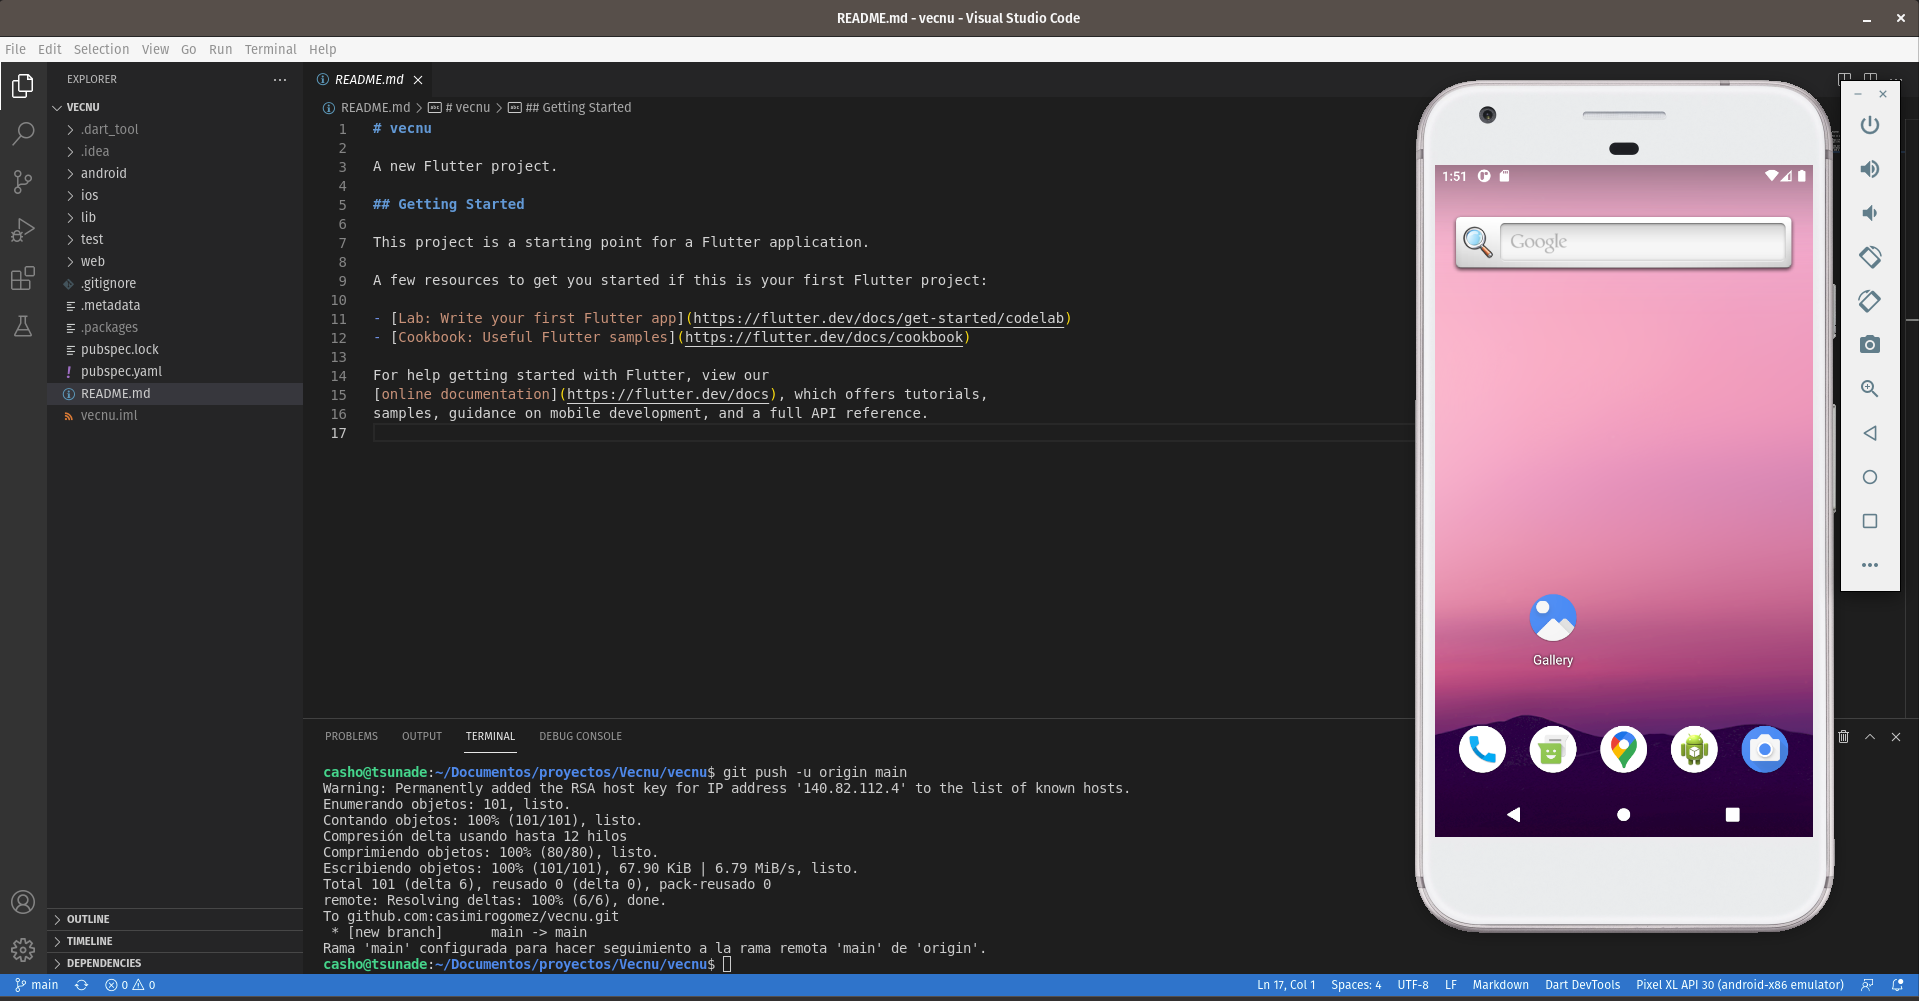
\includegraphics[width=0.7\textwidth]{capitulo1/emulador_1.png}
\caption{Programa creado y editando en \emph{\textbf{visual studio code}} y mostrando el emulador}
\label{cap1:001}
\end{figure} 

Para empezar a trabajar con el proyecto activamos la opción de debug, para ellos nuevamente apretamos las teclas \textbf{ctr->shift-> p} y escribimos \textbf{Debug: Start Debugging}, lo cual nos permite ejecutar nuestro proyecto en el emulador previamente abierto.

\begin{figure}[htb]
\centering
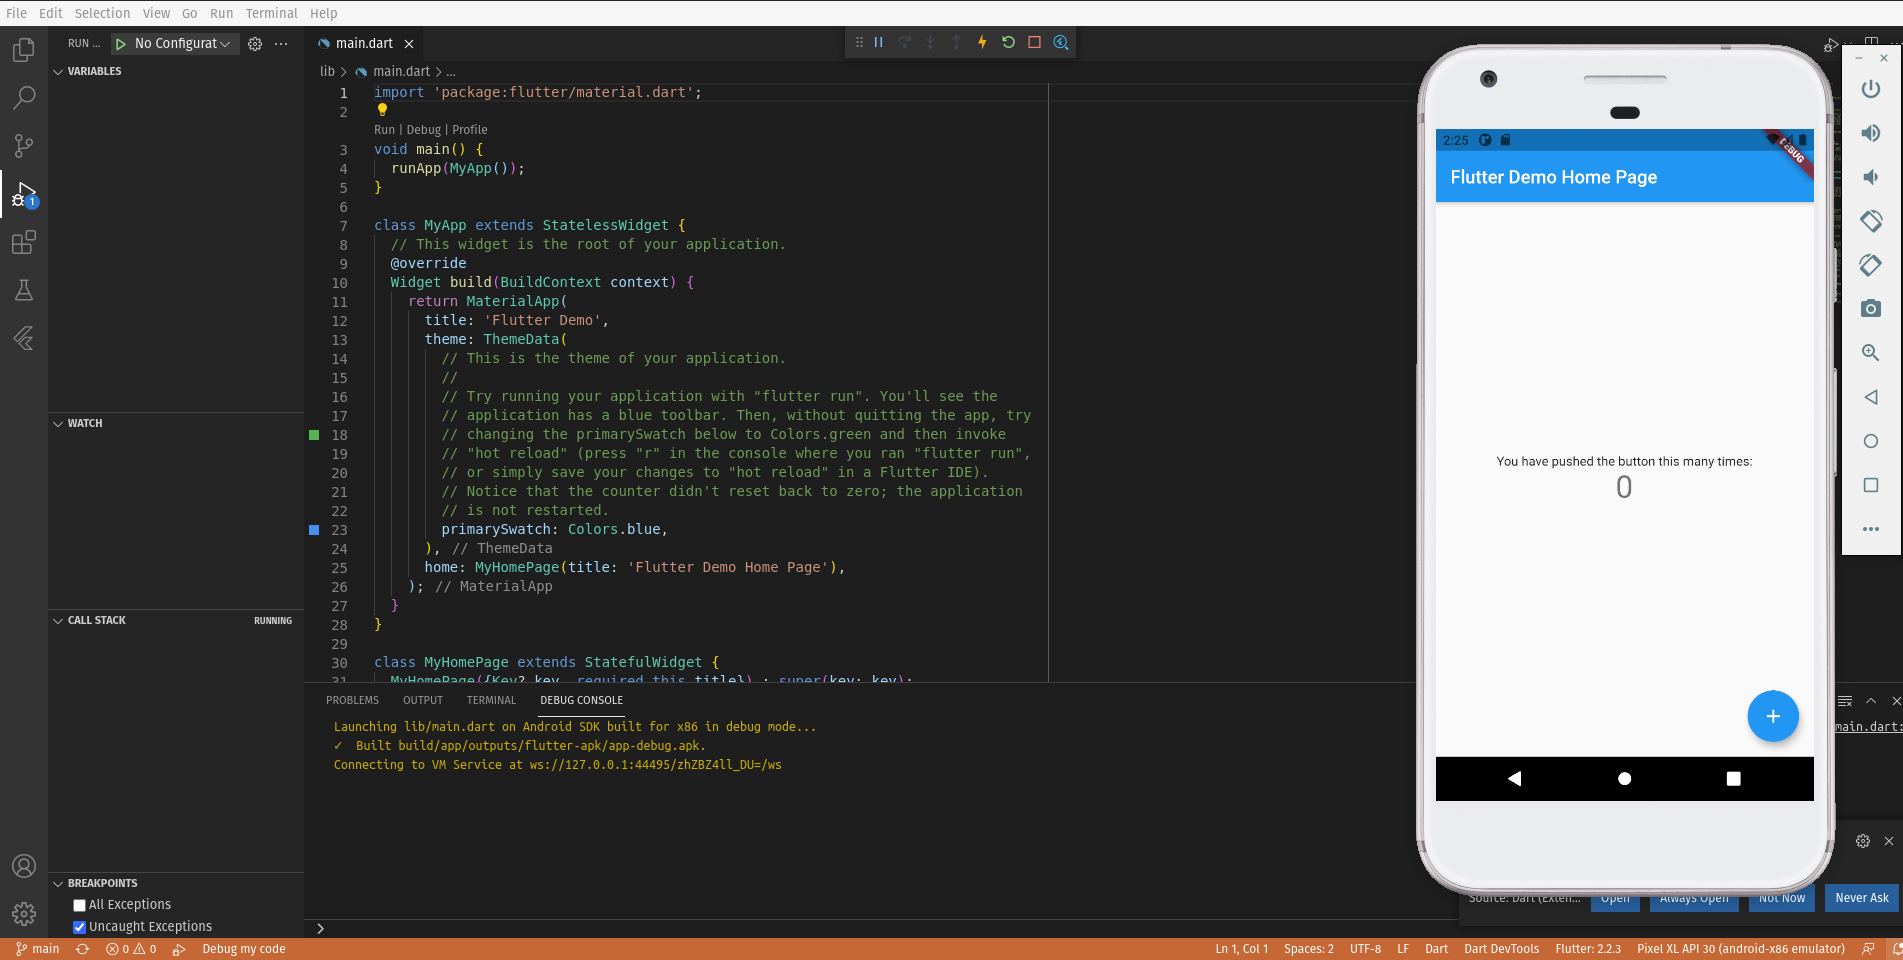
\includegraphics[width=0.6\textwidth]{capitulo1/emulador_corriendo.png}
\caption{Programa ejecutandose en el emulador}
\label{cap1:002}
\end{figure} 

Para que el debugger se ejecute correctamente necesitamos tener instalado Java en nuestra distribución de linux.

\section{Creando los temas para nuestro proyecto}

Para probar como se verán los colores en nuestra aplicación se usa la herramienta \textbf{Material Design Color Tool} la cual se encuentra en la dirección \emph{https://material.io /resources /color/ } en donde se seleccionan los colores primarios y secundarios para nuestra aplicación. En el caso de SMARTEST en la figura \ref{cap1:003} se muestra el código de colores.

\begin{figure}[htb]
\centering
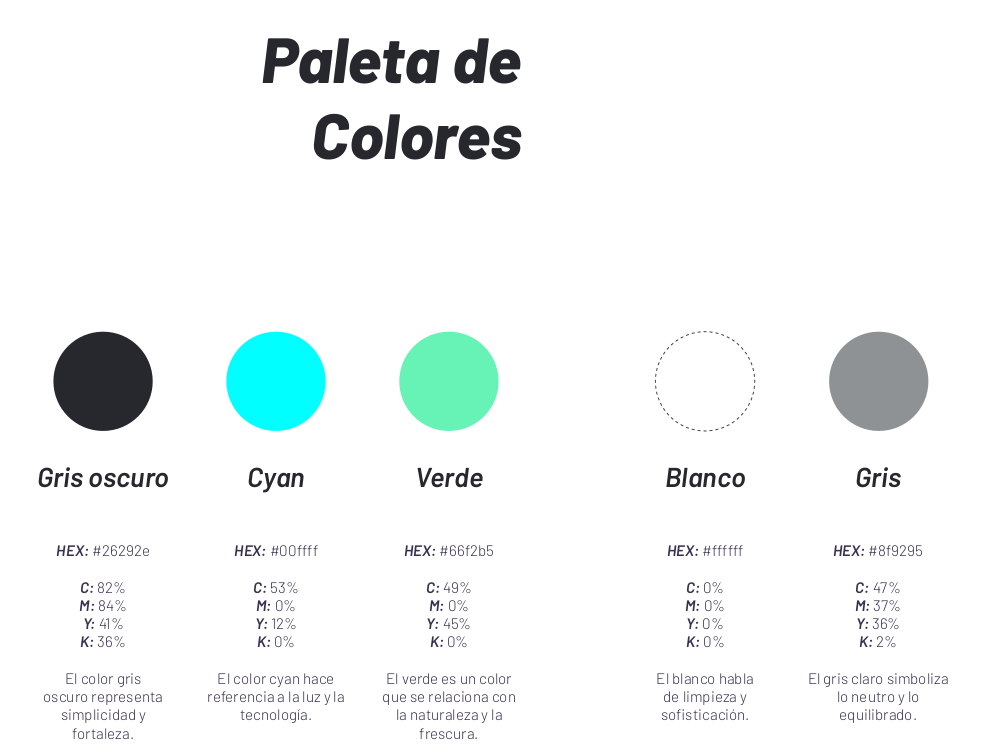
\includegraphics[width=0.6\textwidth]{capitulo1/paleta.png}
\caption{Paleta de colores}
\label{cap1:003}
\end{figure} 

De la figura \ref{cap1:003} se toman dos colores el cyan y el gris, y se forman los colores de la aplicación. Una vez decididos los colores de la aplicación y probados en la página. Se procede a programar el app.

\begin{figure}[htb]
\centering
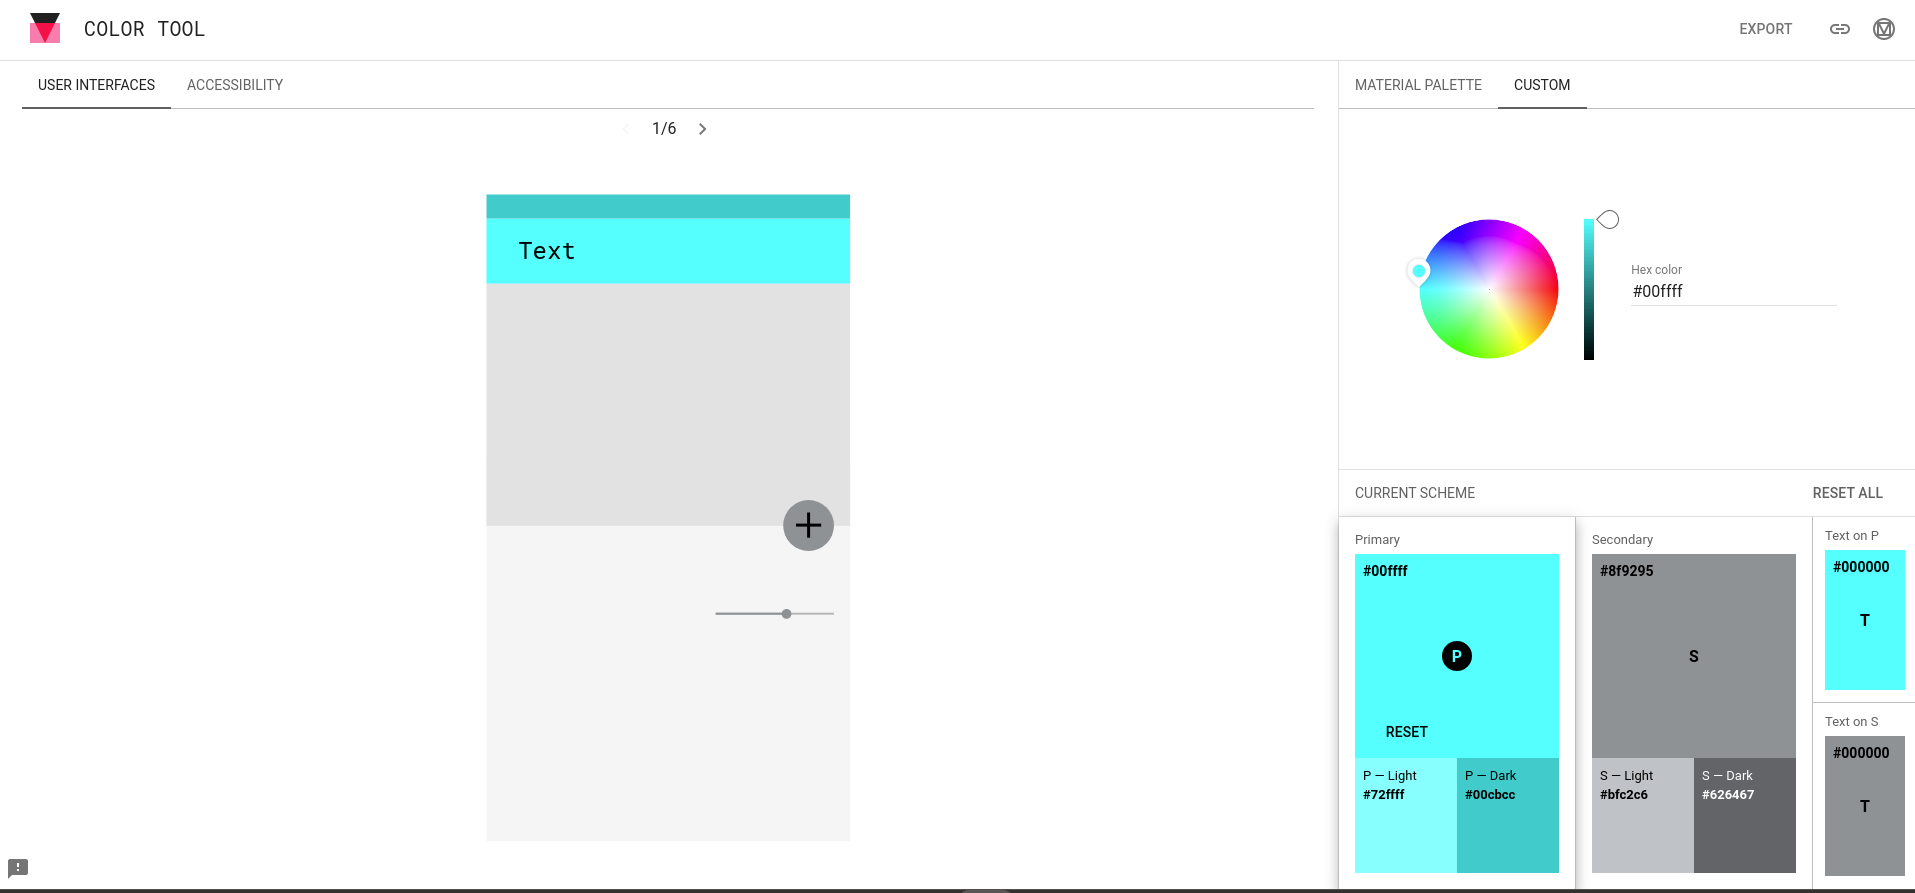
\includegraphics[width=0.5\textwidth]{capitulo1/paleta_primaria.png}
\caption{Colores primario y secundario de la aplicación}
\label{cap1:004}
\end{figure} 

Para ello editamos el archivo \textbf{lib/main.dart} quedando de la siguiente forma

\begin{lstlisting}[language=bash]
...
  @override
  Widget build(BuildContext context) {
    return MaterialApp(
      title: 'Flutter Demo',
      theme: ThemeData(
          brightness: Brightness.dark,
          primaryColor: Colors.cyan[400],
          accentColor: Colors.grey[200],
          textTheme: TextTheme(
              headline5: TextStyle(fontSize: 72.0, fontWeight: FontWeight.bold),
              headline6: TextStyle(fontSize: 36.0, fontStyle: FontStyle.italic),
              bodyText1: TextStyle(fontSize: 18.0))),
      home: MyHomePage(title: 'Flutter Demo Home Page'),
    );
  }
 ...
\end{lstlisting}

Para que el estilo de textos definidos se apliquen a los textos del app necesitamos modificarlos de la siguiente forma:

\begin{lstlisting}[language=java]
...
          children: <Widget>[
            Text(
              'You have pushed the button this many times:',
              style: Theme.of(context).textTheme.bodyText1,
            ),
            Text(
              '$_counter',
              style: Theme.of(context).textTheme.headline4,
            ),
          ],
...
\end{lstlisting}

\section{Construyendo la página de registro}
 
Para construir la página de registro, editamos primero el archivo \textbf{lib /main.dart} y le pondremos el nombre de nuestro e-commerce.

\begin{lstlisting}[language=java]
...
  @override
  Widget build(BuildContext context) {
    return MaterialApp(
      title: 'Vecnu SMARTEST e-commerce',
      theme: ThemeData(
          brightness: Brightness.dark,
          primaryColor: Colors.cyan[400],
          accentColor: Colors.grey[200],
          textTheme: TextTheme(
              headline5: TextStyle(fontSize: 72.0, fontWeight: FontWeight.bold),
              headline6: TextStyle(fontSize: 36.0, fontStyle: FontStyle.italic),
              bodyText1: TextStyle(fontSize: 18.0))),
      //home: MyHomePage(title: 'Flutter Demo Home Page'),
    );
  }
  ...
\end{lstlisting}

En el pedazo de programa de \textbf{lib /main.dart} mostrado anteriormente se realizaron dos modificaciones la primera corresponde al nombre de la aplicación la cual se llamará \textbf{Vecnu SMARTEST e-commerce} y la segunda es que la linea \textbf{home:} se convierte en comentario. La razón para hacer esto es porque vamos a borrar la clase \textbf{MyHomePage} del \textbf{lib /main.dart} y crearemos un nuevo folder en el directorio \textbf{lib} el cual llamaremos \textbf{paginas} y dentro de este directorio crearemos un programa llamado \textbf{lib /paginas /pagina\_registro.dart}

\begin{lstlisting}[language=java]
import 'package:flutter/material.dart';

class PaginaRegistro extends StatefulWidget {
  @override
  PaginaRegistroEstado createState() => PaginaRegistroEstado();
}

class PaginaRegistroEstado extends State<PaginaRegistro> {
  @override
  Widget build(BuildContext context) {
    return Text("Hola Mundo");
  }
}
\end{lstlisting}

Para poder ejecutar el programa creado activamos home: y agragamos la clase \textbf{PaginaRegistro()} anexando asimismo la libreria al programa, quedando de la siguiente manera el programa \textbf{lib /main.dart}.

\begin{lstlisting}[language=java]
import 'package:flutter/material.dart';
import 'package:vecnu/paginas/pagina_registro.dart';

void main() {
  runApp(MyApp());
}

class MyApp extends StatelessWidget {
  // This widget is the root of your application.
  @override
  Widget build(BuildContext context) {
    return MaterialApp(
      title: 'Vecnu SMARTEST e-commerce',
      theme: ThemeData(
          brightness: Brightness.dark,
          primaryColor: Colors.cyan[400],
          accentColor: Colors.grey[200],
          textTheme: TextTheme(
              headline5: TextStyle(fontSize: 72.0, fontWeight: FontWeight.bold),
              headline6: TextStyle(fontSize: 36.0, fontStyle: FontStyle.italic),
              bodyText1: TextStyle(fontSize: 18.0))),
      home: PaginaRegistro(),
    );
  }
}
\end{lstlisting}

Lo cual nos produce una salida que se muestra en la figura \ref{cap1:005}.

\begin{figure}[htb]
\centering
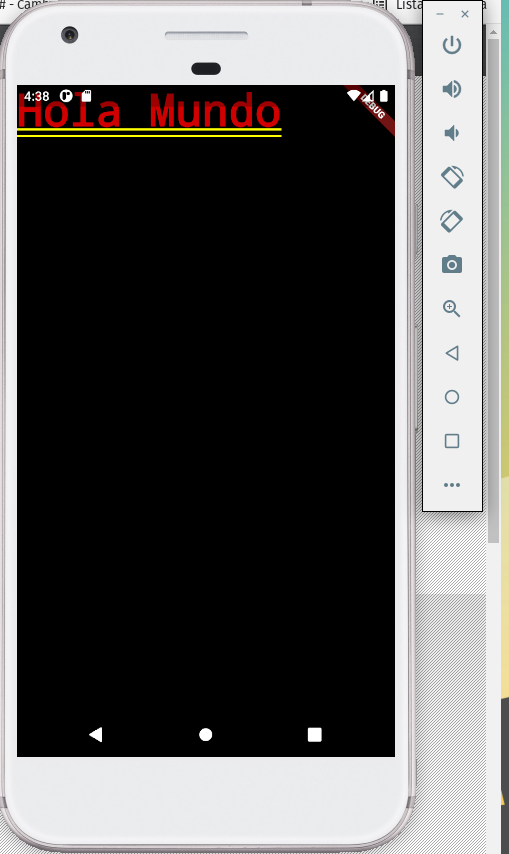
\includegraphics[width=0.3\textwidth]{capitulo1/holaMundo.png}
\caption{Salida del programa Hola Mundo}
\label{cap1:005}
\end{figure} 

\subsection{Creando el Scaffold de la página de registro}

La clase de la página de registro (\textbf{lib /paginas /pagina\_registro.dart}) la editamos y sustituimos el hola mundo por un Scaffold que tiene la estructura que deseamos. 

\begin{lstlisting}[language=java]
import 'package:flutter/material.dart';

class PaginaRegistro extends StatefulWidget {
  @override
  PaginaRegistroEstado createState() => PaginaRegistroEstado();
}

class PaginaRegistroEstado extends State<PaginaRegistro> {
  Widget _mostrarTitulo() {
    return Text(
      'Registro',
      style: Theme.of(context).textTheme.headline5,
    );
  }

  Widget _mostrarEntradaUsuario() {
    return Padding(
        padding: EdgeInsets.only(top: 20.0),
        child: TextFormField(
            decoration: InputDecoration(
                border: OutlineInputBorder(),
                labelText: 'Usuario',
                hintText: 'Introduce usuario, tamano min 6',
                icon: Icon(Icons.face, color: Colors.grey))));
  }

  Widget _mostrarEntradaCorreo() {
    return Padding(
        padding: EdgeInsets.only(top: 20.0),
        child: TextFormField(
            decoration: InputDecoration(
                border: OutlineInputBorder(),
                labelText: 'Correo',
                hintText: 'Introduce un correo valido',
                icon: Icon(Icons.mail, color: Colors.grey))));
  }

  Widget _mostrarEntradaClave() {
    return Padding(
        padding: EdgeInsets.only(top: 20.0),
        child: TextFormField(
            obscureText: true,
            decoration: InputDecoration(
                border: OutlineInputBorder(),
                labelText: 'Clave',
                hintText: 'Introduce clave, tamano min 6',
                icon: Icon(Icons.lock, color: Colors.grey))));
  }

Widget _mostrarAccionesForma() {
    final ButtonStyle raisedButtonStyle = ElevatedButton.styleFrom(
      onPrimary: Colors.black87,
      primary: Theme.of(context).primaryColor,
      minimumSize: Size(88, 36),
      padding: EdgeInsets.symmetric(horizontal: 16),
      shape: const RoundedRectangleBorder(
        borderRadius: BorderRadius.all(Radius.circular(10)),
      ),
    );
    return Padding(
      padding: EdgeInsets.only(top: 20.0),
      child: Column(
        children: [
          ElevatedButton(
            style: raisedButtonStyle,
            child: Text('Enviar',
                style: Theme.of(context)
                    .textTheme
                    .bodyText1!
                    .copyWith(color: Colors.black)),
            onPressed: () => print('Enviado'),
          ),
          TextButton(
            child: Text('Ya te registraste? Entrar'),
            onPressed: () => print('Entrar'),
          )
        ],
      ),
    );
  }


  @override
  Widget build(BuildContext context) {
    return Scaffold(
        appBar: AppBar(title: Text('Registro')),
        body: Container(
          padding: EdgeInsets.symmetric(horizontal: 20.0),
          child: Center(
            child: SingleChildScrollView(
              child: Form(
                child: Column(
                  children: [
                    _mostrarTitulo(),
                    _mostrarEntradaUsuario(),
                    _mostrarEntradaCorreo(),
                    _mostrarEntradaClave(),
                    _mostrarAccionesForma()
                  ],
                ),
              ),
            ),
          ),
        ));
  }
}

\end{lstlisting}

En programa anterior de \textbf{lib /paginas /pagina\_registro.dart} se crean 5 funciones: \_mostrarTitulo(), \_mostrarEntradaUsuario(),\_mostrarEntradaCorreo(), \_mostrarEntradaClave(), \_mostrarAccionesForma(). Todas las funciones regresan un Widget, que crea una columna de Widgets. Cada uno formando el titulo, la entrada de usuario, la entrada de correo, la clave y las formas del boton de enviar y de entrar.

\begin{figure}
\begin{subfigure}{.5\textwidth}
  \centering
  \includegraphics[width=.5\linewidth]{capitulo1/cap1:006.png}
  \caption{Pantalla de registro}
  \label{cap1:006:sfig1}
\end{subfigure}%
\begin{subfigure}{.5\textwidth}
  \centering
  \includegraphics[width=.5\linewidth]{capitulo1/cap1:006:1.png}
  \caption{click en usuario}
  \label{cap1:006:sfig2}
\end{subfigure}
\begin{subfigure}{.5\textwidth}
  \centering
  \includegraphics[width=.5\linewidth]{capitulo1/cap1:006:2.png}
  \caption{click en correo}
  \label{cap1:006:sfig3}
\end{subfigure}
\begin{subfigure}{.5\textwidth}
  \centering
  \includegraphics[width=.5\linewidth]{capitulo1/cap1:006:3.png}
  \caption{click en clave}
  \label{cap1:006:sfig4}
\end{subfigure}
\caption{Imagenes del Funcionamiento de la página de registro}
\label{cap1:006}
\end{figure}

Tambien cuando se pulsa sobre el botón \textbf{enviar} y sobre el botón \textbf{¿Ya te registraste? Entrar} se imprime en la terminal los letreros enviar y entrar 

\begin{figure}[htb]
\centering
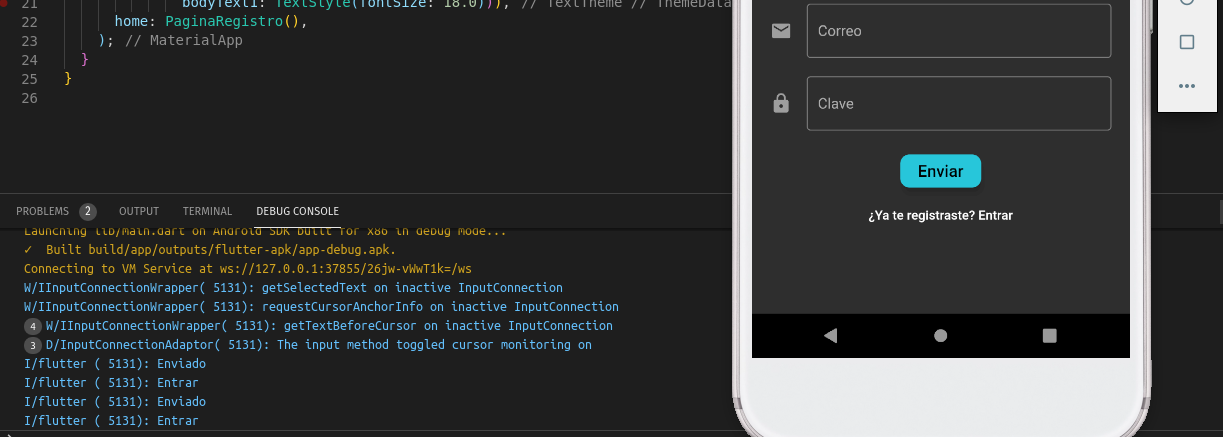
\includegraphics[width=0.5\textwidth]{capitulo1/enviar_entrar.png}
\caption{Salida al pulsar el botón \textbf{enviar} o \textbf{¿ya te registraste? enviar}}
\label{cap1:007}
\end{figure} 


\subsection{Agregando validación de forma, creando estado de forma}

Ahora agregaremos validación a la forma. Primero agregamos validación a la forma de usuario.

\begin{lstlisting}[language=java]
...
  Widget _mostrarEntradaUsuario() {
    return Padding(
        padding: EdgeInsets.only(top: 20.0),
        child: TextFormField(
            validator: (val) => val!.length < 6 ? 'Nombre usuario muy corto': null,
            decoration: InputDecoration(
...
\end{lstlisting}


Posteriormente agregamos validación a la forma de correo

\begin{lstlisting}[language=java]
...
  Widget _mostrarEntradaCorreo() {
    return Padding(
        padding: EdgeInsets.only(top: 20.0),
        child: TextFormField(
            validator: (val) => !val!.contains('@') ? 'Correo invalido':null,
            decoration: InputDecoration(
...
\end{lstlisting}

Ahora agregamos validación a la forma de clave

\begin{lstlisting}[language=java]
...
 Widget _mostrarEntradaClave() {
    return Padding(
        padding: EdgeInsets.only(top: 20.0),
        child: TextFormField(
            validator: (val) => val!.length < 6 ? 'Nombre usuario muy corto': null,
            obscureText: true,
...
\end{lstlisting}



\backmatter
\end{document}
